% Analysis 020: 01_audit_logs.py, 03_figures.py; observations/O004-training-dynamics.md.
\subsection{Retained training dynamics and the finite-budget question}
\label{app:training-dynamics}

We audit A0 and A4-OL1/A7-OL1 at $\kappa=0.5$ at all three sizes.
Each selected condition retains 712 optimizer-boundary records with no
missing interval, gradient overflow or skipped update. The pre-clipping
norm is the global L2 norm of the accumulated, AMP-unscaled task gradient
over all trainable parameters having gradients; it precedes norm-1 clipping
and AdamW. It is neither the post-clipping norm nor OL1's eligible-subset
adaptive direction norm. Task loss is the mean over a boundary's equally
sized microbatches, evaluated before its update. Figure~\ref{fig:training-dynamics}
retains raw curves, aligned by actual input tokens, with the learning-rate
schedules. Successful optimizer calls include the first, zero-learning-rate
boundary, which produces no parameter displacement.

We fix the final 20\% window, steps 570--712, before inspecting its outcomes.
Table~\ref{tab:training-dynamics} gives descriptive OLS slopes of raw task
loss against tokens and median pre-clipping norms over its 143 boundaries.
For A0, the means of the first and last 20 records in this window change
from 5.2750 to 5.2374 at 14M, 4.0506 to 4.0003 at 70M, and 4.5846 to
4.4738 at 410M. Thus all three still improve; the 410M decrease is larger.
Its gradient exceeds the clipping bound on 33 of these 143 boundaries,
versus none for the smaller A0s. Both 410M sparse high-threshold recipes
also continue improving, whereas their 14M curves are nearly flat or
slightly increasing in this window.

\begin{table}[htbp]
\centering\small
\caption{Late-run diagnostics on steps 570--712. Slopes use raw training
task loss per billion input tokens, not validation loss or independent
seed replicates. Sparse recipes use $\kappa=0.5$.}
\label{tab:training-dynamics}
\begin{tabular}{@{}llrr@{}}
\toprule
Size & Recipe & Median pre-clip norm & Loss slope / billion tokens \\
\midrule
14M & A0 & 0.3172 & $-0.1415$ \\
70M & A0 & 0.2950 & $-0.2194$ \\
410M & A0 & 0.8501 & $-0.4448$ \\
14M & A4-OL1 & 0.3651 & $+0.0096$ \\
70M & A4-OL1 & 0.4120 & $-0.0091$ \\
410M & A4-OL1 & 0.4185 & $-0.1318$ \\
14M & A7-OL1 & 0.3303 & $+0.0207$ \\
70M & A7-OL1 & 0.3635 & $-0.0664$ \\
410M & A7-OL1 & 0.4429 & $-0.1051$ \\
\bottomrule
\end{tabular}
\end{table}

These observations are consistent with investigating a finite-budget
limitation, but do not attribute the quality reversal to premature stopping.
Raw norms also depend on parameterization, stochastic gradients and the
optimizer; tokens per parameter and learning rates differ here. Only
validation events at steps 1 and 712 are retained, so there is no late
validation trajectory. A matched continuation of dense and sparse recipes
would be needed to test whether additional training changes their ordering
or their relative penalties. No such continuation is included.

\begin{figure}[tbp]
\centering
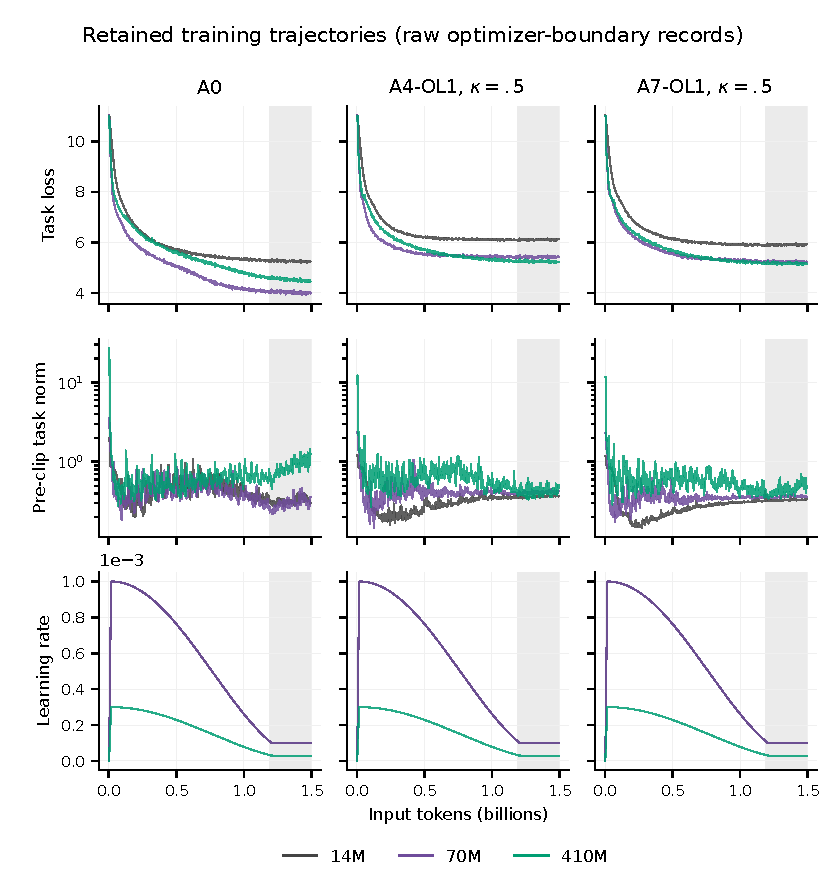
\includegraphics[width=\linewidth]{figures/10-training-dynamics.pdf}
\caption{\textbf{410M dense and high-threshold sparse recipes continue improving late.}
Columns use the same three recipes at each size; rows retain raw task loss,
pre-clipping task-gradient norm (log scale), and learning rate against input
tokens. No smoothing is applied. Shading identifies the fixed final-20\%
window. The 14M and 70M learning-rate curves coincide; 410M uses 30\%
of their peak and minimum rates. All nine curves contain 712 records.}
\label{fig:training-dynamics}
\end{figure}
